% Compile using latex, then dvisvgm --no-fonts --exact.
% Graph: 8 vertices, 14 edges. Its reduced SPQR tree has S=1, P=1, R=2.
% Each tree node contains its skeleton. Dashed edges are virtual.
\documentclass{article}
\usepackage[paperwidth=20cm,paperheight=15cm,margin=1cm]{geometry}
\usepackage{lmodern}
\usepackage{tikz}
\usetikzlibrary{arrows.meta}
\pagestyle{empty}
\definecolor{rigidA}{HTML}{305E7B}
\definecolor{rigidB}{HTML}{934B42}
\definecolor{series}{HTML}{555555}
\newcommand{\rigidskeleton}[4]{%
  \begin{scope}[shift={(#1)},line width=.55pt]
    \node[svertex] (u) at (-.70,-.45) {$0$};
    \node[svertex] (v) at (.70,-.45) {$1$};
    \node[svertex] (a) at (0,.48) {$#2$};
    \node[svertex] (b) at (0,-.10) {$#3$};
    \draw[#4] (u) -- (a) -- (v);
    \draw[#4] (u) -- (b) -- (v);
    \draw[#4] (a) -- (b);
    \draw[#4,dashed] (u) -- (v);
    \node[font=\small] at (0,.88) {$R$};
  \end{scope}
}
\begin{document}
\noindent
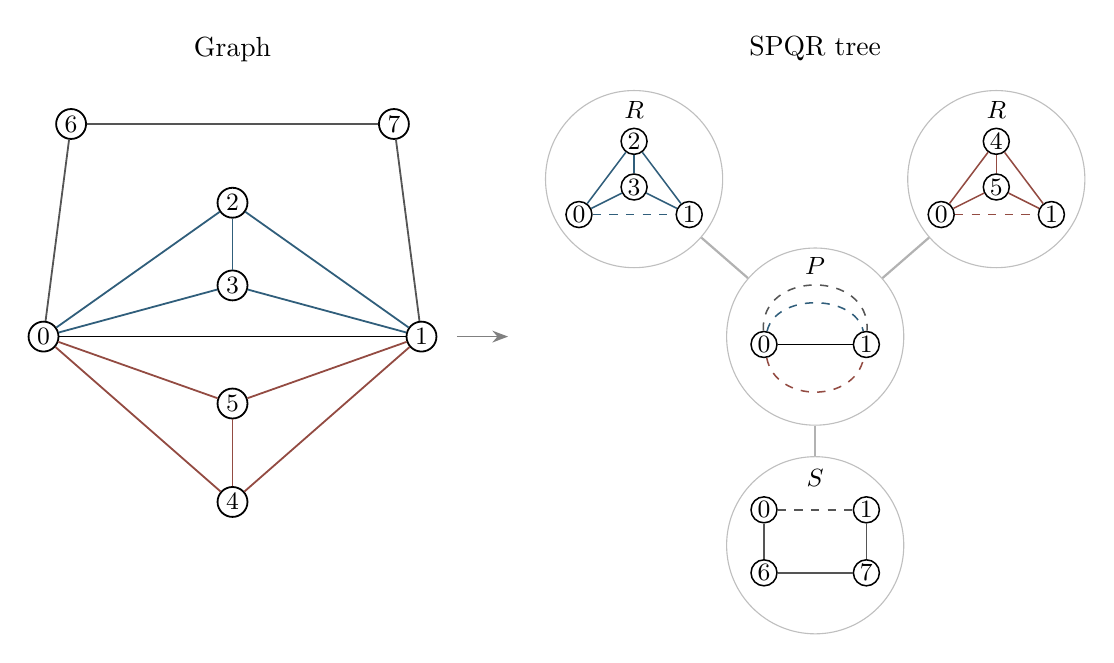
\begin{tikzpicture}[
  line width=.65pt,
  vertex/.style={circle,draw=black,fill=white,minimum size=3.8mm,inner sep=.7pt,font=\small},
  svertex/.style={circle,draw=black,fill=white,minimum size=3.3mm,inner sep=.4pt,font=\small},
  component/.style={circle,draw=gray!50,fill=white,line width=.4pt,minimum size=2.25cm,inner sep=0pt}
]
  \node[font=\normalsize] at (2.4,3.65) {Graph};
  \node[vertex] (g0) at (0,0) {$0$};
  \node[vertex] (g1) at (4.8,0) {$1$};
  \node[vertex] (g2) at (2.4,1.7) {$2$};
  \node[vertex] (g3) at (2.4,.65) {$3$};
  \node[vertex] (g4) at (2.4,-2.1) {$4$};
  \node[vertex] (g5) at (2.4,-.85) {$5$};
  \node[vertex] (g6) at (.35,2.7) {$6$};
  \node[vertex] (g7) at (4.45,2.7) {$7$};
  \draw (g0) -- (g1);
  \draw[rigidA] (g0) -- (g2) -- (g1);
  \draw[rigidA] (g0) -- (g3) -- (g1);
  \draw[rigidA] (g2) -- (g3);
  \draw[rigidB] (g0) -- (g4) -- (g1);
  \draw[rigidB] (g0) -- (g5) -- (g1);
  \draw[rigidB] (g4) -- (g5);
  \draw[series] (g0) -- (g6) -- (g7) -- (g1);

  \draw[-{Stealth[length=2mm]},gray] (5.25,0) -- (5.90,0);

  \node[font=\normalsize] at (9.8,3.65) {SPQR tree};
  \node[component] (Ra) at (7.5,2.0) {};
  \node[component] (Rb) at (12.1,2.0) {};
  \node[component] (P) at (9.8,0) {};
  \node[component] (S) at (9.8,-2.65) {};
  \draw[gray!60,line width=.8pt] (P) -- (Ra);
  \draw[gray!60,line width=.8pt] (P) -- (Rb);
  \draw[gray!60,line width=.8pt] (P) -- (S);

  \rigidskeleton{Ra.center}{2}{3}{rigidA}
  \rigidskeleton{Rb.center}{4}{5}{rigidB}

  \begin{scope}[shift={(P.center)},line width=.55pt]
    \node[svertex] (p0) at (-.65,-.1) {$0$};
    \node[svertex] (p1) at (.65,-.1) {$1$};
    \draw (p0) -- (p1);
    \draw[rigidA,dashed] (p0) .. controls +(.15,.65) and +(-.15,.65) .. (p1);
    \draw[rigidB,dashed] (p0) .. controls +(.15,-.75) and +(-.15,-.75) .. (p1);
    \draw[series,dashed] (p0) .. controls +(-.05,.95) and +(.05,.95) .. (p1);
    \node[font=\small] at (0,.90) {$P$};
  \end{scope}

  \begin{scope}[shift={(S.center)},line width=.55pt]
    \node[svertex] (s0) at (-.65,.45) {$0$};
    \node[svertex] (s1) at (.65,.45) {$1$};
    \node[svertex] (s6) at (-.65,-.35) {$6$};
    \node[svertex] (s7) at (.65,-.35) {$7$};
    \draw[series] (s0) -- (s6) -- (s7) -- (s1);
    \draw[series,dashed] (s0) -- (s1);
    \node[font=\small] at (0,.85) {$S$};
  \end{scope}
\end{tikzpicture}
\end{document}
